% !TeX TS-program = xelatex
\documentclass[aspectratio=169, 12pt, xcolor=table]{beamer}
\usefonttheme{professionalfonts}
\usefonttheme{serif}
\usepackage[T1]{fontenc}
\usepackage{fontspec-xetex}

\usepackage{booktabs}
\usepackage{listings}
\usepackage{subcaption}

\setmainfont{Lato}

%\PassOptionsToPackage[more=table]{xcolor}

% Local configuration
\renewcommand{\figurename}{}
\DeclareCaptionFormat{custom}
{%
	\tiny #3
}
\captionsetup{format=custom}

% Title stuff
\title{Programming}
\subtitle{An Introduction to Python}
\date{Week 01}
\author{Vassilis Markos, Mediterranean College}

\usetheme{streamline}
%\usepackage{/theme/beamerthemestreamline}

% Local Commands
\newcommand{\ohref}[1]{\href{#1}{\texttt{#1}}}

% Code listings

\definecolor{codegreen}{rgb}{0,0.6,0}
\definecolor{codegray}{rgb}{0.5,0.5,0.5}
\definecolor{codepurple}{rgb}{0.58,0,0.82}
\definecolor{backcolour}{rgb}{0.95,0.95,0.92}

\lstdefinestyle{mystyle}{
	backgroundcolor=\color{backcolour},   
	commentstyle=\color{codegreen},
	keywordstyle=\color{magenta},
	numberstyle=\tiny\color{codegray},
	stringstyle=\color{codepurple},
	basicstyle=\ttfamily\footnotesize,
	breakatwhitespace=false,         
	breaklines=true,                 
	captionpos=b,                    
	keepspaces=true,                 
	numbers=left,                    
	numbersep=5pt,                  
	showspaces=false,                
	showstringspaces=false,
	showtabs=false,                  
	tabsize=2
}

\lstset{style=mystyle}

\begin{document}

	\begin{frame}
		\titlepage
	\end{frame}

	\begin{frame}{Contents}
		\tableofcontents
	\end{frame}

	\section{A Brief Intro}\label{sec:a-brief-intro}
	
	\sectionframe
	
	\begin{headsup}{Desperate Times, Desperate Measures}
		\begin{minipage}[t]{0.40\textwidth}
			\vspace{0pt}
			Since we are transitioning on a new platform, things are still a bit quirky. So, to make sure we keep track of who is here and who is not, please \textbf{scan the QR code shown next} or \textbf{click the link below it} and fill in this form with your information (confidential).
		\end{minipage}\hfill
		\begin{minipage}[t]{0.58\textwidth}
			\vspace{0pt}
			\raggedleft
			
\includegraphics[scale=0.35]{./assets/attendance_form.png}
			\centering
			\ohref{https://forms.gle/4yiYhonrjuVs4sCv6}
		\end{minipage}
	\end{headsup}

	\begin{headsup}{Desperate Times, Desperate Measures}
		\begin{minipage}[t]{0.50\textwidth}
			\vspace{0pt}
			For similar reasons, we will also be using a public shared repository to keep our materials as long as our platform is a bit unstable. To visit the platform and download this lecture's materials please use the QR shown right or the link below.
		\end{minipage}\hfill
		\begin{minipage}[t]{0.48\textwidth}
			\vspace{0pt}
			\raggedleft
			
\includegraphics[scale=0.45]{./assets/shared_folder.png}
			\centering
		\end{minipage}
		\vfill
		\begin{scriptsize}
			\ohref{https://github.com/vmarkos-mc/programming}
		\end{scriptsize}
	\end{headsup}

	\begin{headsup}{Some More Technicalities}
		\begin{itemize}
			\item Inside computer labs \textbf{we are not allowed to eat or drink} (coffee included), \textbf{with the exception of water.}
			\item \textbf{Do not try to disassemble any part of the lab equipment!} It might well do so by itself, if needed!
			\item Attendance will be checked \textbf{every hour:}
			\begin{itemize}
				\item Classes start at xx:00 and end at xx:50.
				\item You can enter class with a 10 minutes delay.
				\item You can also enter class after that  allowed 10 minutes delay, but, in this case, you will have been marked as absent.
				\item In case of scheduled absence, please inform me prior to our class via email or in person.
			\end{itemize}
		\end{itemize}
	\end{headsup}
	
	\begin{frame}{\texttt{sudo echo whoami}}
		\begin{itemize}
			\item Vassilis (name) Markos (surname): it also works the other way around.
			\item My interests include: AI / XAI, Quantum Computing, Data Science, Operator Theory, Statistics, Software Development\ldots\ (this might be of your interest too in the future, in case you are looking for a \textbf{thesis supervisor}).
			\item I am mostly a Linux / UNIX user, so, please, be kind towards my ignorance regarding MS Windows. :)
		\end{itemize}
	\end{frame}

	\begin{frame}{What Is This Course?}
		What is this course about? (multiple choice, one correct answer):
		\renewcommand{\theenumi}{\alph{enumi}}
		\begin{enumerate}
			\item Interesting and cool programming stuff.
			\item A good chance to deeply understand Python.
			\item A process where you have to write computer programs.
			\item \textbf{All of the above.}
		\end{enumerate}
		In case you already know Python, don't worry, we will also cover more complex stuff in this course, so, stay tuned!
	\end{frame}

	\begin{headsup}{Module(s) Assessment}
		All coursework will be submitted \textbf{directly on UDO} (you will get your credentials soon if you have not yet). This means that:
		\begin{itemize}
			\item Delayed submissions are not possible (including submissions by email etc).
			\item The only way to get an extension is by formally applying for one \textbf{at the University of Derby.}
			\item All UDO submissions are by default checked by Turnitin.
		\end{itemize}
	\end{headsup}

	\begin{headsup}{Module(s) Assessment}
		So, in order for things to run smoothly:
		\begin{itemize}
			\item You should \textbf{work} on coursework sufficiently \textbf{prior to the deadline!}
			\item In case of extension, \textbf{make sure you have all necessary documents} available, e.g., doctor's written diagnosis, in case of a medical condition.
			\item I will be accepting \textbf{drafts} which can be discussed during \textbf{office hours} to make sure things are okay for submission.
			\item Do not make (excessive) use of Generative AI!
		\end{itemize}
	\end{headsup}

	\begin{frame}{Module's Coursework}
		There is a single--part coursework for this course:
		\begin{itemize}
			\item \textbf{Coursework 1 (100\%):} A programming portfolio including Python programs developed by you covering various topics of this course (flow control, loops, functions, classes, etc).
		\end{itemize}
		
		We will work on your portfolio in class as well as on similar exercises, so, do not worry about difficulty. Just pay attention to the lectures and play around with Python on your own!
	\end{frame}

	\section{What is Python?}\label{sec:what-is-python}
	
	\sectionframe
	
	\begin{frame}{Some Programmer Humour First\ldots}
		\begin{figure}
			\centering
			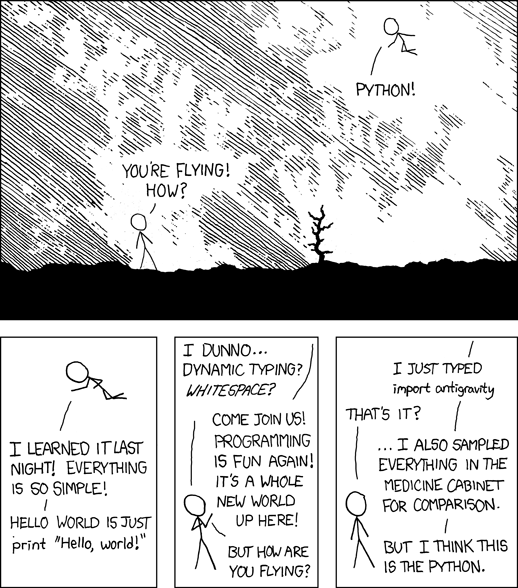
\includegraphics[height=0.65\textheight]{./assets/xkcd_python.png}
			\caption{The moment you understand this is the moment you'll have learnt Python. Source: \ohref{https://xkcd.com/353/}.}
		\end{figure}
	\end{frame}
	
	\begin{frame}{Python in a Nutshell}
		Python is:
		\begin{itemize}
			\item An \textbf{interpreted} language (so, no compiler here). This means that commands are executed sequentially, one after the other.
			\item Quite \textbf{high--level}, which means that it makes several decisions for us, making coding much simpler.
			\item \textbf{Tricky}, because of its high level, since you might think that your code works in some way, while it actually works quite differently.
			\item \textbf{Slow}. Really slow, mostly because it has to make all those decisions for us.
		\end{itemize}
	\end{frame}

	\begin{frame}{The Compilation Process (in general)}%
		\begin{minipage}[t]{0.68\textwidth}%
			\vspace{0pt}%
			\begin{itemize}
				\item \textbf{Source File:} The code file we write on a PC.
				\item \textbf{Object File:} The compiled code file, usually machine / CPU instructions (e.g., assembly).
				\item \textbf{Executable:} A file that can be executed by a certain Operating System (OS).
				\item \textbf{Compiler:} A computer program that transforms a source file to an object file.
				\item \textbf{Linker:} A computer program that interconnects a source file with other required existing programs (libraries).
			\end{itemize}
		\end{minipage}\hfill%
		%
		\begin{minipage}[t]{0.3\textwidth}%
			\vspace{0pt}
			\centering
			\begin{tikzpicture}
			\pgfmathsetmacro{\dy}{-1.5}
			\node[rectangle, draw=black] (source) at (0,0) {Source File(s)};
			\node[rectangle, draw=black] (object) at (0,1*\dy) {Object File(s)};
			\node[rectangle, draw=black] (exe) at (0,2*\dy) {Executable};
			\node[rectangle, draw=black] (prog) at (0,3*\dy) {Program (RAM)};
			\draw[thick, ->] (source) -- (object) node[pos=0.5, right] {\small Compiler};
			\draw[thick, ->] (object) -- (exe) node[pos=0.5, right] {\small Linker};
			\draw[thick, ->] (exe) -- (prog) node[pos=0.5, right] {\small OS};
			\end{tikzpicture}
		\end{minipage}
	\end{frame}

	\begin{frame}{The Interpretation Process (in general)}
		\begin{minipage}[t]{0.50\textwidth}
			\vspace{0pt}
			\raggedright
			The interpretation process is more straightforward:
			\begin{itemize}
				\item The interpreter consumes \texttt{x = 5} and executes it.
				\item The interpreter consumes \texttt{y = 7} and executes it.
				\item The interpreter consumes \texttt{z = x + y} and executes it.
				\item The interpreter consumes \texttt{print(z)} and executes it.
			\end{itemize}
		\end{minipage}\hfill
		\begin{minipage}[t]{0.48\textwidth}
			\vspace{0pt}
			\centering
			\lstinputlisting[language=Python]{../source/interpreter_sample.py}
		\end{minipage}
	\end{frame}

	\begin{irrelevant}{The Bare Truth}
		Python is not actually interpreted; it is \textbf{compiled and then interpreted:}
		\begin{itemize}
			\item Python code is first \textbf{compiled} to Python bytecode, i.e., a lower level code generated by Python's compiler.
			\item Then, this bytecode is:
			\begin{itemize}
				\item either \textbf{interpreted} by a Python interpreter, or;
				\item \textbf{compiled}, by a python bytecode compiler.
			\end{itemize}
			\item In general, whether a certain language is interpreted or compiled is not a feature of the language per se but of the \textbf{implementation} of the language. For an interesting discussion of that:
		\end{itemize}%
		\begin{center}%
			\vspace{-0.71\topsep}
			\ohref{https://stackoverflow.com/a/6889798/12461122}
		\end{center}
	\end{irrelevant}

	\begin{frame}{Installing Python}
		In order to play around with Python you need to install it:
		\begin{itemize}
			\item Avoid installing Python 2.x, as it is no longer supported. \textbf{Install Python 3.8 or later}, instead.
			\item For MS Windows, you can find the corresponding releases here: \ohref{https://www.python.org/downloads/windows/}
			\item For Linux / Unix Python is probably already installed, however you can follow the instructions found here: \ohref{https://docs.python-guide.org/starting/install3/linux/}
			\item You can also use online interpreters, which I would discourage you to, since we will sooner or later need to work on our own machine.
		\end{itemize}
	\end{frame}

	\begin{frame}{Installing a Text Editor}
		In order to write some Python code you need a text editor:
		\begin{itemize}
			\item \textbf{You cannot use MS Word} or some other similar editor.
			\item One popular choice is MS \textbf{Visual Studio Code} with any relevant plugins. We will be using this in our classes as it is quite convenient.
			\item You can download it from: \ohref{https://code.visualstudio.com/}.
			\item You can also choose any other editor / programming environment, like \textbf{PyCharm}.
		\end{itemize} 
	\end{frame}

	\begin{frame}{Configuring VSCode Plugins}
		\begin{minipage}[t]{0.50\textwidth}
			\vspace{0pt}
			To install python plugins:
			\begin{itemize}
				\item Click on the ``four squares'' icon on the left sidebar.
				\item Write ``python'' in the search bar.
				\item Install the two first plugins, ``Python'' and ``Python Debugger'', as shown right.
			\end{itemize}
		\end{minipage}\hfill
		\begin{minipage}[t]{0.48\textwidth}
			\vspace{0pt}
			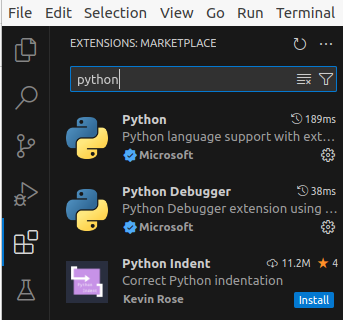
\includegraphics[width=\textwidth]{./assets/vsc_plugins.png}
		\end{minipage}
	\end{frame}

	\begin{frame}{Running Python Code in VSCode}
		\begin{minipage}[t]{0.65\textwidth}
			\vspace{0pt}
			\raggedright
			To execute a Python program simply press the ``Play'' button on the top right of the editor (see right). Any results should be displayed at the bottom of your window, as shown below.
		\end{minipage}\hfill
		\begin{minipage}[t]{0.33\textwidth}
			\vspace{0pt}
			\centering
			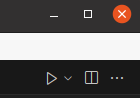
\includegraphics[width=0.5\textwidth]{./assets/vsc_run.png}
		\end{minipage}\vfill
		\begin{minipage}{\textwidth}
			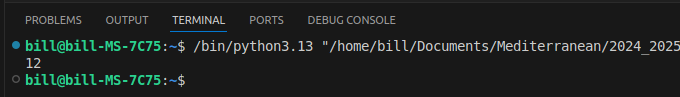
\includegraphics[width=\textwidth]{./assets/vsc_output.png}
		\end{minipage}
	\end{frame}

	\begin{headsup}{PATH Variables}
		Regardless of your Operating System (OS), you have to be really careful with PATH variables:
		\begin{itemize}
			\item Such variables inform your OS where to look for Python (and other stuff).
			\item For Windows, when installing Python check the box that asks you whether to append Python to the PATH.
			\item Instructions for Windows, Linux and Mac may be found here: \ohref{https://realpython.com/add-python-to-path/}
		\end{itemize}
	\end{headsup}

	\section{Getting Started With Python}\label{sec:getting-started-with-python}
	
	\sectionframe
	
	\begin{frame}{\texttt{hello\_world.py}}
		It is usual to start a course in programming by presenting a simple program which prints ``Hello, world!'' on our console. So, let's write this in Python!
		\lstinputlisting[language=Python]{../source/hello_world.py}
		Execute the above program! Does it work as expected?
	\end{frame}

	\begin{frame}{Some Operations}
		\begin{minipage}[t]{0.5\textwidth}
			\vspace{0pt}
			Right you can see a simple Python program.
			\begin{itemize}
				\item Without executing it, can you guess what will be printed on your screen?
				\item Execute it and verify your conjecture.
				\item Explain what those peculiar \texttt{+} and \texttt{*} do.
			\end{itemize}
		\end{minipage}\hfill
		\begin{minipage}[t]{.45\textwidth}
			\vspace{0pt}
			\centering
			\lstinputlisting[language=Python]{../source/magic_001.py}
		\end{minipage}	
	\end{frame}

	\begin{frame}{More Operations}
		\begin{minipage}[t]{0.5\textwidth}
			\vspace{0pt}
			Right you can see a simple Python program.
			\begin{itemize}
				\item Without executing it, can you guess what will be printed on your screen?
				\item Execute it and verify your conjecture.
				\item Explain how \texttt{**} works.
			\end{itemize}
		\end{minipage}\hfill
		\begin{minipage}[t]{.45\textwidth}
			\vspace{0pt}
			\centering
			\lstinputlisting[language=Python]{../source/magic_002.py}
		\end{minipage}	
	\end{frame}

	\begin{frame}{More Operations}
		\begin{minipage}[t]{0.5\textwidth}
			\vspace{0pt}
			Right you can see a simple Python program.
			\begin{itemize}
				\item Without executing it, can you guess what will be printed on your screen?
				\item Execute it and verify your conjecture.
				\item Explain what's the difference between \texttt{/}, \texttt{//}, and \texttt{\%}.
			\end{itemize}
		\end{minipage}\hfill
		\begin{minipage}[t]{.45\textwidth}
			\vspace{0pt}
			\centering
			\lstinputlisting[language=Python]{../source/magic_003.py}
		\end{minipage}	
	\end{frame}

	\begin{frame}{More Operations}
		\begin{minipage}[t]{0.5\textwidth}
			\vspace{0pt}
			Right you can see a simple Python program.
			\begin{itemize}
				\item Without executing it, can you guess what will be printed on your screen?
				\item Execute it and verify your conjecture.
				\item Explain why the program works the way it does.
			\end{itemize}
		\end{minipage}\hfill
		\begin{minipage}[t]{.45\textwidth}
			\vspace{0pt}
			\centering
			\lstinputlisting[language=Python]{../source/magic_004.py}
		\end{minipage}	
	\end{frame}

	\begin{frame}{What About \texttt{=} and \texttt{==}?}
		\begin{minipage}[t]{0.5\textwidth}
			\vspace{0pt}
			Right you can see a simple Python program.
			\begin{itemize}
				\item Without executing it, can you guess what will be printed on your screen?
				\item Execute it and verify your conjecture.
				\item Explain why the program works the way it does.
			\end{itemize}
		\end{minipage}\hfill
		\begin{minipage}[t]{.45\textwidth}
			\vspace{0pt}
			\centering
			\lstinputlisting[language=Python]{../source/magic_005.py}
		\end{minipage}	
	\end{frame}

	\begin{frame}{Summarising Our Observations}
		\centering
		\begin{tabular}{lp{0.75\textwidth}}
			\toprule%
			\textbf{Operator} & \textbf{Description} \\\midrule
			\texttt{+}, \texttt{-}, \texttt{*}, \texttt{/}, \texttt{**} & Addition, subtraction, multiplication, division and power operators.\\%
			\texttt{//}, \texttt{\%} & Integer division and modulus (remainder) operators.\\
			\texttt{==} & Comparison operator (equality)\\%
			\texttt{<}, \texttt{>}, \texttt{<=}, \texttt{>=} & Comparison operators (inequalities, as in maths)\\%
			\bottomrule
		\end{tabular}
	\end{frame}

	\begin{frame}{What's Your Type?}
		Run the following program on your PC. What does it print? Can you explain its output (or, even better, guess it)?
		\lstinputlisting[language=Python]{../source/data_types.py}
	\end{frame}

	\begin{frame}{Python Data Types}
		\centering
		\begin{tabular}{lp{0.5\textwidth}l}
			\toprule%
			\textbf{Type} & \textbf{Description} & \textbf{Example}\\\midrule%
			\texttt{int} & Represents integer numbers & \texttt{-5}, \texttt{0}, \texttt{82}\\%
			\texttt{float} & Represents floating point numbers & \texttt{-6.54}, \texttt{4.0}, \texttt{89.2}\\%
			\texttt{string} & Represents sequences of printable characters & \texttt{"foo"}, \texttt{"Python is FUN"}\\%
			\texttt{bool} & Represents one of the two available Boolean values & \texttt{True}, \texttt{False}\\%
			\bottomrule
		\end{tabular}
	\end{frame}

	\begin{frame}{Reading User Input}
		So far, we have printed stuff on screen, but it would be nice to ask the user for some input, in order to make our programs more interactive. This can be achieved with Python's \texttt{input}, as in the following example (run it on your machine):
		\lstinputlisting[language=Python]{../source/read_input.py}
		Can you explain what happened?
	\end{frame}

	\begin{frame}{What About Non--String Input?}
		What if we want to read something that is not a string? For instance, execute the following program:
		\lstinputlisting[language=Python]{../source/kaboom.py}
		What did happen? What does the output read? How can we fix that?
	\end{frame}

	\begin{frame}{Becoming a Developer}
		You must see something like the following:
		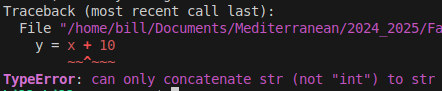
\includegraphics[width=0.8\textwidth]{./assets/type_error.png}
		\begin{itemize}
			\item Let us look online for what other developers have to say\ldots
			\item Write on some search engine the main message of your error: \texttt{TypeError:\ can only concatenate str (not "int") to str}
			\item How can we fix this?
		\end{itemize}
	\end{frame}

	\begin{frame}{Python Errors}
		In Python, a \texttt{TypeError} usually refers to an error regarding some misuse of data types.
		\begin{itemize}
			\item In our case, as you must have found online, the error is about the data type returned by \texttt{input()}.
			\item \texttt{input()} by default returns a \textbf{string}.
			\item So, in order to handle its input as a number, say an integer, we should \textbf{cast it to an integer}.
			\item This can be done with the help of Python's function \texttt{int()}, which takes a Python object, e.g., a string, and returns an integer, if possible, or raises an error, otherwise.
		\end{itemize}
	\end{frame}

	\begin{frame}{Handling Non--String Input}
		The correct way to parse user input as an integer is as follows:
		\lstinputlisting[language=Python]{../source/noboom.py}
		What we did above was to wrap \texttt{input()} with \texttt{int()}, so \texttt{int()} parses its output and converts it to an integer.
	\end{frame}

	\begin{frame}{Python's Casting Functions}
		\begin{tabular}{lp{0.7\textwidth}}
			\toprule%
			\textbf{Function} & \textbf{Description}\\\midrule%
			\texttt{int()} & Casts its argument to an \textbf{integer}, if possible, or raises a \texttt{ValueError}.\\%
			\texttt{float()} & Casts its argument to a \textbf{float}, if possible, or raises a \texttt{ValueError}.\\%
			\texttt{str()} & Casts its argument to a \textbf{string}, if possible, or raises a \texttt{ValueError}.\\%
			\texttt{bool()} & Casts its argument to a \textbf{boolean} value, if possible, or raises a \texttt{ValueError}.\\%
			\bottomrule
		\end{tabular}
	\end{frame}

	\begin{frame}{This, and this, or that, but not the other\ldots}
		\begin{itemize}
			\item How would you express in Python the following?
			\begin{quote}
				``A number, $x$, is greater than 5.''
			\end{quote}
			\item One possible python expression could be: \texttt{x > 5}.
			\item How about that?
			\begin{quote}
				``A number, $x$, is less than 12.''
			\end{quote}
			\item Similarly, it could be: \texttt{x < 12}.
			\item How about that?
			\begin{quote}
				``A number, $x$, is greater than 5 and less than 12.''
			\end{quote}
		\end{itemize}
	\end{frame}

	\begin{frame}{Composite Logical Expressions}
		\begin{itemize}
			\item In Python, such composite logical expressions are written with the help of \textbf{logical operators}.
			\item Logical operators are the same as mathematical operators (\texttt{+}, \texttt{-}, \texttt{*}, \texttt{/}, etc) just for boolean values instead of numbers.
			\item The following program checks whether a number is between 5 and 12 (run this a few times with various inputs):
		\end{itemize}
		\lstinputlisting[language=Python]{../source/composite_conditions_001.py}
	\end{frame}

	\begin{frame}{Python Logical Operators}
		\centering
		\begin{tabular}{lp{0.7\textwidth}}
			\toprule%
			\textbf{Operator} & \textbf{Description}\\\midrule%
			\texttt{and} & Corresponds to ``both'' in everyday language.\\%
			\texttt{or} & Corresponds to an ``inclusive'' or, i.e., \textbf{either one of the two options or both} may hold.\\%
			\texttt{not} & Corresponds to everyday language's ``not'' (negation).\\%
			\bottomrule
		\end{tabular}
	\end{frame}

	\begin{frame}{How Do Logical Operators Work?}
		Fill in the following table with the values you think each operator yields in each case. You can draw inspiration from your everyday experience:
		\vfill
		\centering\rowcolors{2}{streamlinegray}{white}%
		\setlength{\tabcolsep}{14pt}
		\begin{tabular}{ccccc}
			\toprule
			\texttt{x} & \texttt{y} & \texttt{\textbf{not} x} & \texttt{x \textbf{and} y} & \texttt{x \textbf{or} y}\\\midrule
			\texttt{True} & \texttt{True} & & & \\
			\texttt{True} & \texttt{False} & & & \\
			\texttt{False} & \texttt{True} & & & \\
			\texttt{False} & \texttt{False} & & & \\%
			\bottomrule
		\end{tabular}
		\vfill
	\end{frame}

	\begin{frame}{Testing Your Conjecture}
		Fill in the following table using Python to evaluate each expression (write a small program that does this for each case):
		\vfill
		\centering\rowcolors{2}{streamlinegray}{white}%
		\setlength{\tabcolsep}{14pt}
		\begin{tabular}{ccccc}
			\toprule
			\texttt{x} & \texttt{y} & \texttt{\textbf{not} x} & \texttt{x \textbf{and} y} & \texttt{x \textbf{or} y}\\\midrule
			\texttt{True} & \texttt{True} & & & \\
			\texttt{True} & \texttt{False} & & & \\
			\texttt{False} & \texttt{True} & & & \\
			\texttt{False} & \texttt{False} & & & \\%
			\bottomrule
		\end{tabular}
		\vfill
		\raggedright
		Compare Python's view of logical operators with yours. What do you observe?
	\end{frame}

	\begin{frame}{Python + Logical Operators}
		The values Python assigns to those expressions are:
		
		\vfill
		\centering\rowcolors{2}{streamlinegray}{white}%
		\setlength{\tabcolsep}{14pt}
		\begin{tabular}{ccccc}
			\toprule
			\texttt{x} & \texttt{y} & \texttt{\textbf{not} x} & \texttt{x \textbf{and} y} & \texttt{x \textbf{or} y}\\\midrule
			\texttt{True} & \texttt{True} & \texttt{False} & \texttt{True} & \texttt{True} \\
			\texttt{True} & \texttt{False} & \texttt{False} & \texttt{False} & \texttt{True} \\
			\texttt{False} & \texttt{True} & \texttt{True} & \texttt{False} & \texttt{True} \\
			\texttt{False} & \texttt{False} & \texttt{True} & \texttt{False }& \texttt{False} \\%
			\bottomrule
		\end{tabular}
		\vfill
	\end{frame}

	\begin{frame}{Useful Resources}
		There are several high quality Python resources around the web:
		\begin{itemize}
			\item Usually quite in depth and informative tutorials can be found at: \ohref{https://realpython.com/}. I highly recommend this as a source for your personal learning.
			\item The official Python Tutorial, while quite lengthy, goes in great detail to cover all interesting and useful features of the language: \ohref{https://docs.python.org/3/tutorial/index.html}
			\item There is also a great (and long) video tutorial available on YouTube: \ohref{https://www.youtube.com/watch?v=rfscVS0vtbw}
		\end{itemize}
	\end{frame}

	\section{Fun Time!}\label{sec:fun-time}
	
	\sectionframe
	
	\begin{frame}{In--class Exercise \#001}
		A foot (imperial distance unit, not part of one's body) is equal to 0.3048 metres.
		\begin{enumerate}
			\item Write a python program that asks the user a distance in feet and prints on screen the same distance in metres.
			\item Write another python program that asks the user a distance in metres and prints on screen the same distance in feet.
		\end{enumerate}
		Test your programs by running them for multiple inputs!
	\end{frame}

	\begin{frame}{In--class Exercise \#002}
		Write a Python program that:
		\begin{itemize}
			\item Asks the user to provide two integer numbers, let $m$ and $n$.
			\item Checks if $m$ divides $n$.
			\item Prints ``Divisor!'' if $m$ divides $n$ and ``Not Divisor!'' otherwise.
		\end{itemize}
		Test your program by running it for multiple inputs!
		
		\textit{This requires Python machinery we have not discussed yet, so, The Internet is your friend!}
	\end{frame}

	\begin{frame}{In--class Exercise \#003}
		Write a Python program that:
		\begin{itemize}
			\item Asks the user to provide two integer numbers, let $m$ and $n$.
			\item Checks if $m$ divides $n$ and $m^2$ does not divide $n$.
			\item Prints ``Simple Divisor!'' if the above holds and ``Non--simple Divisor!'' otherwise.
		\end{itemize}
		Test your program by running it for multiple inputs!
		
		\textit{This requires Python machinery we have not discussed yet, so, The Internet is your friend!}
	\end{frame}

	\begin{frame}{In--class Exercise \#004}
		Run the following Python program:
		\lstinputlisting[language=Python]{../source/tabbing.py}
		What is the console output? Try to make it work as intended!
	\end{frame}

	\begin{frame}{In--class Exercise \#005}
		For which values of \texttt{x} does the following program print \texttt{True} and for which \texttt{False} (do not run it!):
		\lstinputlisting[language=Python]{../source/bar.py}
		Run the program. Did it work as you expected? Explain why it works that way.
	\end{frame}

	\begin{frame}{In--class Exercise \#006}
		What input should you give in the following program in order to print \texttt{False}?
		\lstinputlisting[language=Python]{../source/foo.py}
		Explain your answer in detail!
	\end{frame}

	\begin{frame}{In--class Exercise \#007}
		Write a Python program that:
		\begin{itemize}
			\item Asks the user to provide to floats, $a$, and $b$.
			\item Stores the value of $a$ to $b$ and that of $b$ to $a$.
			\item Prints the new values of $a$ and $b$.
		\end{itemize}
		Explain your chain of thought in detail.
	\end{frame}

	\begin{frame}{Homework 1}
		As your homework, you will have to explore some features of Python we have not yet explored in class. To do so, you will have to follow this \textbf{excellent tutorial:}
		\begin{center}
			\small\vspace{-1.2\topsep}
			\ohref{https://realpython.com/courses/basics-conditional-logic-control-flow/}
		\end{center}
		Take time to \textbf{watch all short videos} / read the transcripts (whichever you prefer) and \textbf{solve all provided exercises.} Share any thoughts, questions, your solutions to the tutorials problems and anything else (relevant) via email at: \texttt{v.markos@mc-class.gr}.
	\end{frame}

	\begin{frame}{Homework 2}
		This is a more advanced homework, building on top of the previous one. So, start working on this one once (and if) you are done with the previous one. Otherwise, don't worry, we will cover much of that material in the following lectures. Given that, start working on the following tutorial:
		\begin{center}
			\footnotesize\vspace{-1.2\topsep}
			\ohref{https://realpython.com/courses/conditional-logic-control-flow-exercises/}
		\end{center}
		Share anything relevant at: \texttt{v.markos@mc-class.gr}.
	\end{frame}

	\begin{frame}{Any Questions?}
		\begin{minipage}{0.35\textwidth}
			\raggedright
			Do not forget to fill in the questionnaire shown right!
		\end{minipage}\hfill
		\begin{minipage}{0.58\textwidth}
			\vspace{0pt}
			\raggedleft
			
\includegraphics[scale=0.4]{./assets/post_lesson_assessment.png}
			\centering
			\ohref{https://forms.gle/dKSrmE1VRVWqxBGZA}
		\end{minipage}
	\end{frame}
	
\end{document}